%!TEX root = ../Thesis.tex

\chapter{Fahrspur-Bestimmung aus Trajektorie-Clustern}
\label{cha:lane_definition}
% Cluster-Bereinigung: Entfernen von Outliern (Spurwechselvorgänge)
%   Beschreibung Probleme: Performance, Zuverlässigkeit (initial Distanzbasiert, erweitert Dichtebasiert --> Ähnliche Ergebnisse und Performance)
%   Verfahren mit evtl. besseren Resultaten noch aufwendiger und basierend meist auf selben Ideen (Distanzmaße, Dichten etc.)
% Bestimmung Referenz-Trajektorie
% Bestimmung von Spur-Envelopes
% Partitionierung der initialen Spur-Schätzungen
% Alignment der Spuren

In diesem Kapitel wird beschrieben, wie aus den bereits identifizierten Trajektorie-Clustern
Geometrie-Informationen der Fahrspuren abgeleitet werden. Hierzu sind primär drei Schritte notwendig:
Bestimmung der Spur-Mittellinien, Bestimmung der Spurhüllen und anschließend die Partitionierung sich überlagernder
Spuren. Hinzu kommen weitere kleine Schritte, welche ebenfalls nachfolgend beschrieben werden.

\section{Ausfilterung von Spurwechselvorgängen}
\label{sec:real2_filter_lane_change}
% Warum?
% Wie?
% Probleme, andere Lösungen und deren Nachteile

Bevor mithilfe der im vorherigen Schritt gewonnenen Trajektorie-Cluster Mittellinien von Fahrspuren bestimmt
werden können, müssen diese nochmals vorverarbeitet werden. Die einzelnen Cluster enthalten teilweise
Bewegungsbahnen, welche Spurwechselvorgänge beinhalten. Diese Trajektorien müssen, so weit wie möglich,
entfernt werden, da sie die anschließende Geometrie-Bestimmung negativ beeinträchtigen. Die Trajektorien
eines Clusters sollten eindeutig einer realen Fahrspur zuzuordnen sein. In Abbildung
\ref{fig:real2_clusters_pre_postpro} sind beispielhaft zwei Cluster dargestellt, welche eine Vielzahl an
Spurwechselvorgängen enthalten.

\begin{figure}[H]
    \centering
    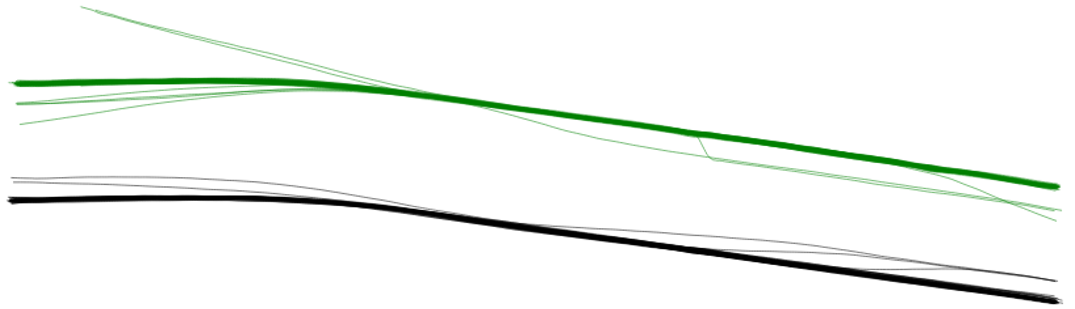
\includegraphics[width=0.8\linewidth]{../resources/img/umsetzung/U2/Clusters_Pre_Postprocessing}
    \caption{Trajektorie-Cluster mit Spurwechselvorgängen}
    \label{fig:real2_clusters_pre_postpro}
\end{figure}

Die Grundidee, welche der Ausfilterung der Spurwechselvorgänge zugrunde liegt, ist, jene Trajektorien
aus einem Cluster zu entfernen, welche eine überdurchschnittlich hohe mittlere Distanz zu allen anderen
Trajektorien des Clusters besitzen. Als Distanzmaß wird erneut die LCSS Distanz verwendet.
Ein ähnlicher, Distanz-basierter Ausreißer-Detektionsansatz wird auch in \cite[]{Mirge2017} vorgestellt.
Der verwendete Algorithmus ist in Listing \ref{lst:pseudo_post_processing} beschrieben.

\begin{lstlisting}[caption=Pseudocode Cluster Post-Processing, language=Pseudo, label=lst:pseudo_post_processing]
algorithm filterCluster:
  input:  unfiltered trajectories of cluster: trasIn
  output: filtered trajectories of cluster

  meanTrajectoryDistances :=
    for each traj in trasIn do
      yield mean LCSS distance of traj to all other trajectories of trasIn
    end

  clusterCmpVal := select median of meanTrajectoryDistances as comparison value

  resultTrajs :=
    for each traj in trasIn do
      if meanDist of traj < 1.5 * clusterCmpVal then
        yield trajs
      end
    end

  return resultTrajs
\end{lstlisting}

Das beschriebene Verfahren ist einfach, eignet sich aber gut, um das gewünschte Ziel zu erreichen.
Die in Abbildung \ref{fig:real2_clusters_post_postpro} dargestellten Ergebnisse zeigen dies.
Aus den in Abbildung \ref{fig:real2_clusters_pre_postpro} enthaltenen Trajektorie-Clustern wurden alle
Spurwechselvorgänge und Ausreißer entfernt. Die Effektivität konnte auch bei Anwendung auf andere Datensätze
bestätigt werden.

\begin{figure}[H]
    \centering
    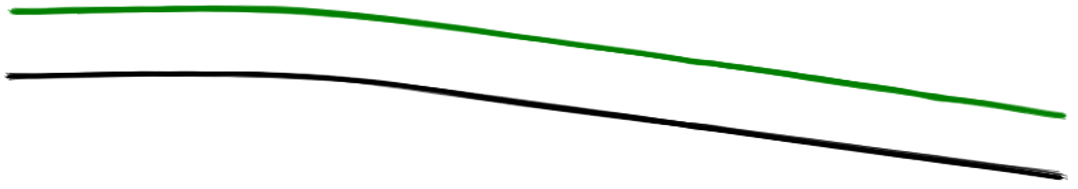
\includegraphics[width=0.8\linewidth]{../resources/img/umsetzung/U2/Clusters_Post_Postprocessing}
    \caption{Trajektorie-Cluster ohne Spurwechselvorgänge}
    \label{fig:real2_clusters_post_postpro}
\end{figure}

Zu beachten ist allerdings auch, dass die Zeitkomplexität des Verfahrens bei großen Trajektorie-Clustern
nicht unerheblich ist. Dies ist auf die Komplexität des LCSS Distanzmaßes zurückzuführen.
Bei der Untersuchung alternativer Vorgehensweise wurde allerdings klar, dass es grundlegend schwer ist,
dieses Problem performant zu lösen. In \cite[]{Meng2018} werden hierzu diverse Distanz- und Dichte-basierte
Arbeiten vorgestellt und verglichen. Da diese alle allerdings nicht weniger komplex sind und häufig
die verfolgten Ziele über die hier geforderten hinausgehen, wurde entschieden den oben beschriebenen Ansatz
beizubehalten. Durch die Parallelisierung der Berechnung der mittleren Abstände konnte die Performance
des Ansatzes außerdem deutlich gesteigert werden.

\section{Bestimmung Spurmittellinien}
\label{sec:real2_define_lane_centerline}

% Warum nicht Traj. mit min avg Distanz zu anderen?
% Vorgehen
% Ergebnisse

\section{Bestimmung Spurhüllen}
\label{sec:real2_define_lane_envelope}

% Erklärung SpurDefinition (LaneEstimate) Über Nodes? Siehe Rel. Work.
% Bestimmung benachbarter Spuren
% Bestimmung paralleler Spuren
% Bestimmung des mittleren Abstands zwischen zwei parallelen Spurpaaren
% Bestimmung Envelope-Punkte

\section{Partitionierung von Fahrspuren}
\label{sec:real2_lane_partitioning}

% Arbeiten nur noch mit LaneEstimates
% Grundidee: Sich überschneidende Spuren an Schnittpunkte partitionieren
% Problem: welche Spur ganz lassen und welche partitionieren
% Aufteilung in drei Spur-Typen (isolated, primary, secundary)
% Finden von sich überlappenden Spurpaaren
% Entscheidung für zu partitionierende Spuren (nach Kriterien)
% Partitionierung